\chapter{存储}

\section{磁盘扩容}
磁盘扩容需要几个必要的条件:
\begin{itemize}
  \item 扩容的分区是lvm
  \item 存在未使用的空余磁盘或者分区
\end{itemize}

\subsection{LVM的基本概念}
LVM主要涉及以下几个概念:
\begin{itemize}
  \item PV(Physical Volume),物理卷:物理卷在逻辑卷管理中处于最底层,它可以是实际物理硬盘上的分区,也可以是整个物理硬盘,也可以是raid设备
  \item VG(Volumne Group),卷组:建立在物理卷之上,一个卷组中至少要包括一个物理卷,在卷组建立之后可动态添加物理卷到卷组中。一个逻辑卷管理系统工程中可以只有一个卷组,也可以拥有多个卷组。
  \item LV(Logical Volume),逻辑卷:逻辑卷建立在卷组之上,卷组中的未分配空间可以用于建立新的逻辑卷,逻辑卷建立后可以动态地扩展和缩小空间。系统中的多个逻辑卷可以属于同一个卷组,也可以属于不同的多个卷组。
  \item PE(Physical Extent),物理块:LVM 默认使用4MB的PE区块,而LVM的LV最多仅能含有65534个PE (lvm1 的格式),因此默认的LVM的LV最大容量为4M*65534/(1024M/G)=256G。PE是整个LVM 最小的储存区块,也就是说,其实我们的资料都是由写入PE 来处理的。简单的说,这个PE 就有点像文件系统里面的block 大小。所以调整PE 会影响到LVM 的最大容量!不过,在 CentOS 6.x 以后,由于直接使用 lvm2 的各项格式功能,因此这个限制已经不存在了。
\end{itemize}

PV,VG和LV的关系如图 \colorunderlineref{fig:lvm}所示
\begin{figure}[H]
  \centering
  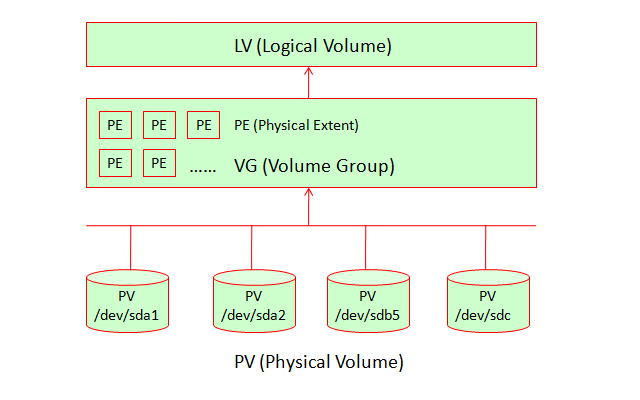
\includegraphics[width=\linewidth]{lvm.png}
  \caption{关系图}
  \label{fig:lvm}
\end{figure}

\subsection{扩容的基本步骤}
\begin{outline}[enumerate]
  \1 创建pv
\begin{code-in-enumerate}{bash}
pvcreate /dev/vdb
\end{code-in-enumerate}

  \1 查看pv
\begin{code-in-enumerate}{bash}
pvscan
pvs
\end{code-in-enumerate}

  \1 查看并选择需要扩容的vg
\begin{code-in-enumerate}{bash}
vgscan
vgs
\end{code-in-enumerate}

  \1 扩容vg
\begin{code-in-enumerate}{bash}
vgextend rhel /dev/vdb
\end{code-in-enumerate}

  \1 确认vg扩容成功
\begin{code-in-enumerate}{bash}
vgs
\end{code-in-enumerate}

  \1 查看lvm
\begin{code-in-enumerate}{bash}
lvs
\end{code-in-enumerate}

  \1 扩容lvm
\begin{code-in-enumerate}{bash}
lvextend -l +100%FREE /dev/rhel/root
\end{code-in-enumerate}

  \1 扩容文件系统

      Lvm扩容之后,必须需要文件系统识别才行,因此,如果扩容lvm,则一般要进行文件系统的扩容。
      针对extx类型的文件系统
\begin{code-in-enumerate}{bash}
resize2fs -p /dev/rhel/root
\end{code-in-enumerate}

      针对xfs类型的文件系统
\begin{code-in-enumerate}{bash}
xfs_growfs /dev/rhel/root
\end{code-in-enumerate}

\end{outline}
完整的操作如图 \colorunderlineref{fig:extendlvm}所示
\begin{figure}[H]
  \centering
  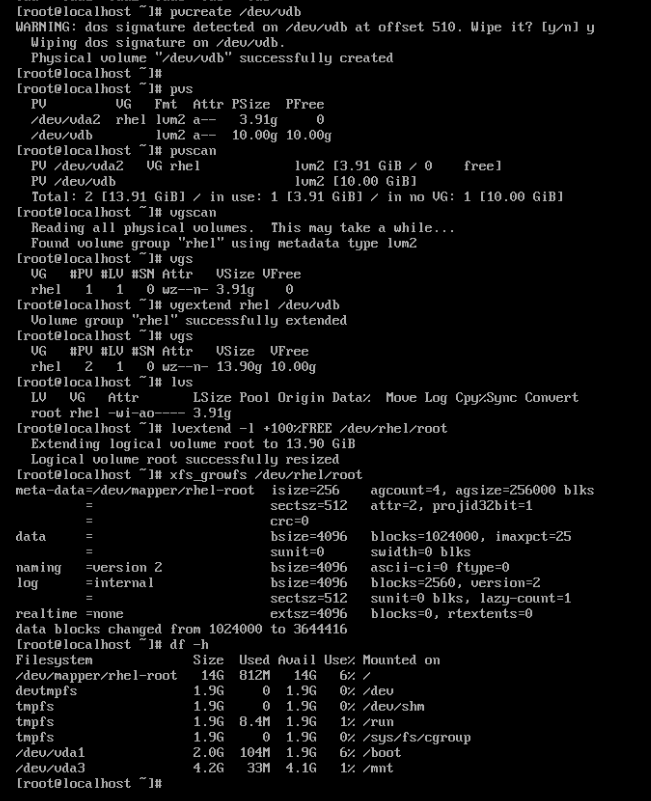
\includegraphics[scale=0.3]{extendlvm.png}
  \caption{磁盘根分区扩容}
  \label{fig:extendlvm}
\end{figure}
